\documentclass[uplatex]{jsarticle}

\usepackage{mylatex}
\usepackage{ap3}
\usepackage{ascmac}


\title{応用プログラミングⅢ [Q2] レポート}
\author{C0115114 菅野路哉}
\date{2016年6月9日}

\usepackage[dvipdfmx]{graphicx}
\begin{document}
\maketitle
% --- main content ---

\section{目的}
デザインパターンの一種であるFactoryMethodについて、課題を通して理解する。FactoryMethodを用いたプログラムを作成し、どのような場面で利用されているのかを調べ、具体例をあげて説明する。

\section{課題}
\figref{uml}に示すプログラムを完成させる。このプログラムは、ゲームのキャラクターに名前をつけるときに利用されるといったものである。\pgref{main}では、{\tt RetroFactory}で作成した2つのゲームキャラクターに対して{\tt show()}メソッドを呼び出し、キャラクターの名前を表示している。\pgref{result}では、設定した名前の英数字が全て大文字に変わっているのが分かる。


次に、作成した{\tt en06.framework}パッケージを用いて、{\tt en06.front}パッケージに{\tt OldFactory}クラスを作成する。{\tt OldFactory}メソッドを用いた場合の実行結果を\pgref{result2}に示す。{\tt OldFactory}クラスを用いたキャラクタは、名前の英数字が全て大文字に変わったうえ、名前の長さが4文字に短縮される。

\begin{figure}[h]
  \begin{center}
    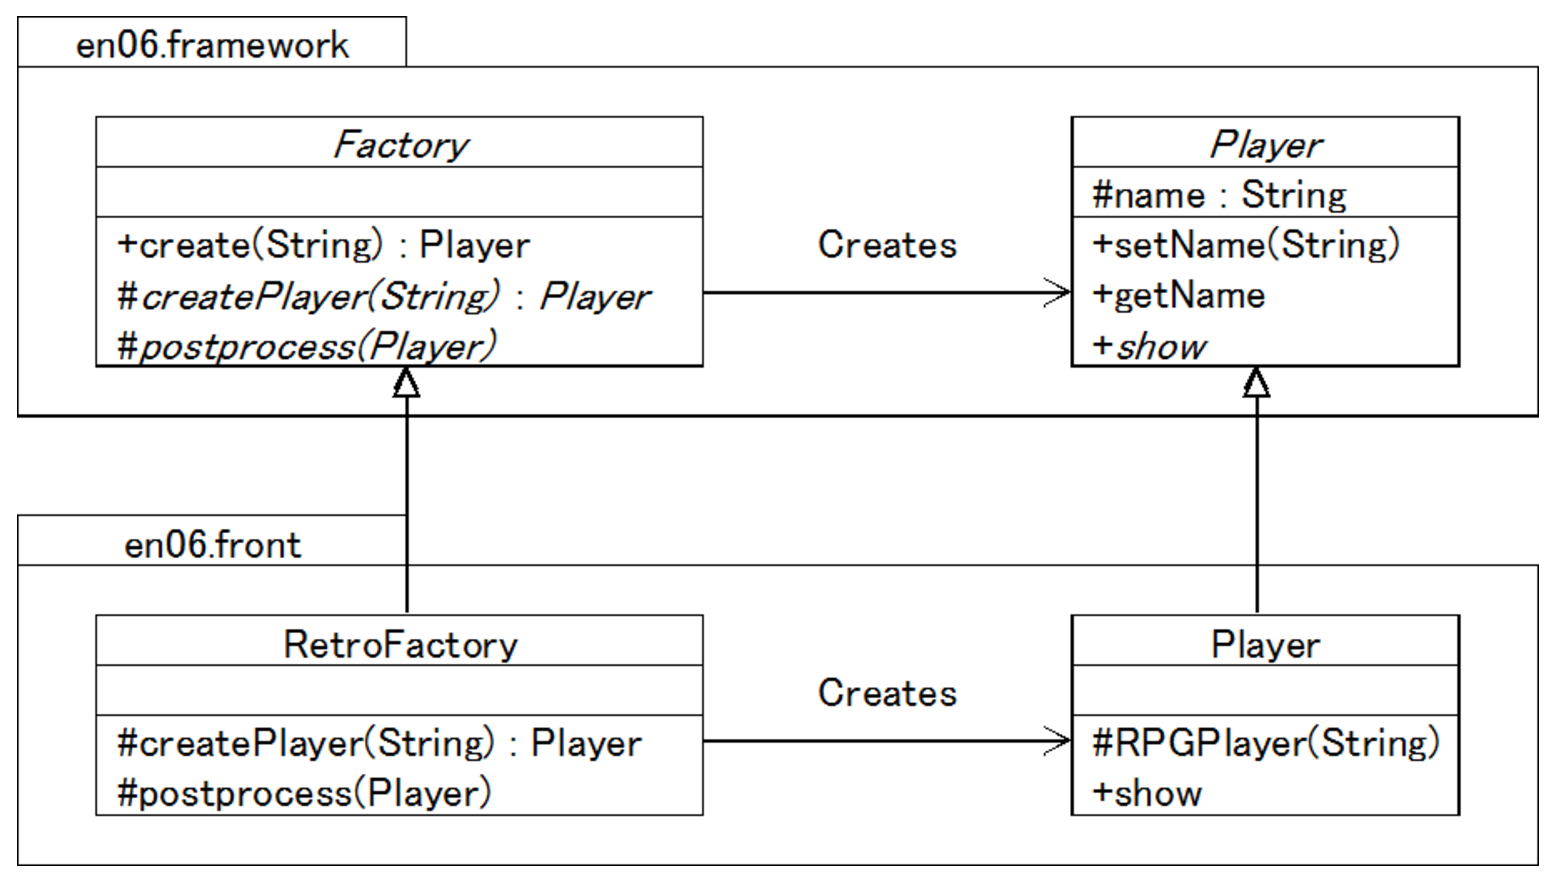
\includegraphics[width=0.8\linewidth]{uml.eps}
    \caption{作成するクラス図}
    \label{uml}
  \end{center}
\end{figure}

\newpage

\section{ソースコード}
\subsection{{\tt Factory}}
\lstinputlisting[
  caption=Factory.java,
  label=src1,
  language=Java
]{./src/en06/framework/Factory.java}

\subsection{{\tt Player}}
\lstinputlisting[
  caption=Player.java,
  label=src2,
  language=Java
]{./src/en06/framework/Player.java}

\subsection{{\tt RetroFactory}}
\lstinputlisting[
  caption=RetroFactory.java,
  label=src3,
  language=Java
]{./src/en06/front/RetroFactory.java}

\newpage

\subsection{{\tt RPGPlayer}}
\lstinputlisting[
  caption=RPGPlayer.java,
  label=src4,
  language=Java
]{./src/en06/front/RPGPlayer.java}

\subsection{{\tt OldFactory}}
\lstinputlisting[
  caption=OldFactory.java,
  label=src5,
  language=Java
]{./src/en06/front/OldFactory.java}

\newpage

\subsection{実行ファイル}
\lstinputlisting[
  caption=Main.java,
  label=main,
  language=Java
]{./src/en06/Main.java}

\lstinputlisting[
  caption=Main2.java,
  label=main2,
  language=Java
]{./src/en06/Main2.java}

\section{実行結果}
\lstinputlisting[
  caption={\tt Main.java}の実行結果,
  label=result,
  numbers=none
]{./src/en06/result.txt}

\lstinputlisting[
  caption={\tt Main2.java}の実行結果,
  label=result2,
  numbers=none
]{./src/en06/result2.txt}

\section{解説}
\pgref{src1}では、Playerを生成するFactoryの抽象クラスを定義した。このクラスは、{\tt createPlayer}メソッドによって、Playerオブジェクトを生成し、{\tt postprocess}メソッドによって、生成されたPlayerオブジェクトに対して追加処理を行い、それを生成物として返すという流れを用いてインスタンスの生成を行う。インスタンスの生成を行う際は、{\tt create}メソッドを用いる。


\pgref{src2}では、Factoryによって生成されるオブジェクトを定義した。このクラスに定義されている{\tt setName}メソッドは、引数にキャラクターの名前を取り、その名前をフィールドの{\tt name}に格納する。{\tt getName}メソッドでは、フィールドの{\tt name}に格納されている情報を戻り値とする。{\tt show}メソッドでは、何らかの情報を表示させることを目的に抽象メソッドとして定義した。


\pgref{src3}では、Factoryクラスの実装を行った。このクラスは、{\tt createPlayer}メソッドで生成するオブジェクトの定義と、{\tt postprocess}メソッドで行う追加処理の定義を行った。{\tt createPlayer}メソッドでは、{\tt RPGPlayer}の生成のみを行う。{\tt postprocess}メソッドでは、キャラクターの名前を大文字に変換する処理を行う。


\pgref{src4}では、Playerクラスの実装を行った。このクラスは、コンストラクタの引数にキャラクター名を定義してあり、Playerクラスに実装してある{\tt setName}メソッドを用いて、nameフィールドに名前を格納する。次に、{\tt show}メソッドの実装を行った。{\tt show}メソッドでは、{\tt Name: }の表示を付与しつつ、キャラクターの名前を表示する。


\pgref{src5}では、Factoryクラスの実装を行った。このクラスは、{\tt createPlayer}メソッドで生成するオブジェクトの定義と、{\tt postprocess}メソッドで行う追加処理の定義を行った。{\tt createPlayer}メソッドでは、{\tt RPGPlayer}の生成のみを行う。{\tt postprocess}メソッドでは、キャラクターの名前を大文字に変換する処理を行い、先頭4文字のみにする処理を行う。


\pgref{main}では、RetroFactoryを用いたプログラムの実行を行った。初めに、{\tt RetroFactory}のインスタンスを生成し、そのインスタンスから、{\tt create}メソッドを使用してキャラクターのインスタンスを生成する。最後に、{\tt show}メソッドを用いてキャラクターの情報を表示する。


\pgref{main2}では、OldFactoryを用いたプログラムの実行を行った。\pgref{main}から変更すべき点は、6行目でimportしているものの変更と、9行目で作成するインスタンスの変更のみである。


\section{考察・まとめ}
{\tt FactoryMethod}は、インスタンス生成時に、複雑な同様の処理が必要になる場合に使用される。この複雑な処理の手順を定義しておけば、インスタンス生成時には、この処理を記す必要が無くなり、安全性が保証される。


{\tt FactoryMethod}が使用されている例を挙げると、{\tt java}内で{\tt FactoryMethod}は、{\tt javaScript}を使用する際に必要となる{\tt ScriptEngine}の作成に使用されている。この場合、{\tt Factory}に当たる機能は、{\tt ScriptEngineFactory}と、{\tt ScriptEngineManager}の二種がある。{\tt ScriptEngine}を生成するための{\tt Factory}機能が{\tt ScriptEngineFactory}であり、{\tt ScriptEngineFactory}を生成するための{\tt Factory}機能が{\tt ScriptEngineManager}となっている。{\tt ScriptEngine}のインスタンス生成時には、{\tt ScriptEngineManager}の引数に言語名を渡して{\tt getEngineByName}メソッドを呼び出す。この時に、{\tt ScriptEngine}の{\tt Factory}の生成や、その{\tt Factory}の存在確認、{\tt null}の確認、スコープの設定、{\tt Exception}の生成が定義されているため、それらを意識する必要が無くなっている。

% --- main content ---
\end{document}
